\documentclass[12pt]{article}
\usepackage[utf8]{inputenc}
\usepackage[spanish,es-lcroman, es-tabla]{babel}
\usepackage[autostyle,spanish=mexican]{csquotes}
\usepackage{amsmath}
\usepackage{amssymb}
\usepackage{nccmath}
\numberwithin{equation}{section}
\usepackage{amsthm}
\usepackage{graphicx}
\usepackage{epstopdf}
\DeclareGraphicsExtensions{.pdf,.png,.jpg,.eps}
\usepackage{color}
\usepackage{float}
\usepackage{multicol}
\usepackage{enumerate}
\usepackage[shortlabels]{enumitem}
\usepackage{anyfontsize}
\usepackage{anysize}
\usepackage{array}
\usepackage{multirow}
\usepackage{enumitem}
\usepackage{cancel}
\usepackage{tikz}
\usepackage{circuitikz}
\usepackage{tikz-3dplot}
\usetikzlibrary{babel}
\usepackage{bm}
\usepackage{mathtools}
\usepackage{esvect}
\usepackage{hyperref}
\usepackage{relsize}
\usepackage{siunitx}
\usepackage{physics}
%\usepackage{biblatex}
\usepackage{standalone}
\usepackage{mathrsfs}
\usepackage{bigints}
\usepackage{bookmark}
\spanishdecimal{.}

\setlist[enumerate]{itemsep=0mm}

\renewcommand{\baselinestretch}{1.5}

\let\oldbibliography\thebibliography

\renewcommand{\thebibliography}[1]{\oldbibliography{#1}

\setlength{\itemsep}{0pt}}
%\marginsize{1.5cm}{1.5cm}{2cm}{2cm}


\newtheorem{defi}{{\it Definición}}[section]
\newtheorem{teo}{{\it Teorema}}[section]
\newtheorem{ejemplo}{{\it Ejemplo}}[section]
\newtheorem{propiedad}{{\it Propiedad}}[section]
\newtheorem{lema}{{\it Lema}}[section]

\usepackage{titling}
\setlength{\jot}{12pt}
\title{Polinomios de Hermite \\ {\large Tema 5 - Matemáticas Avanzadas de la Física}\vspace{-2.5\baselineskip}}
\author{}
\date{}
\begin{document}
\maketitle
\fontsize{14}{14}\selectfont

\begin{table}[hbt!]
\centering
\begin{tabular}{l l}
$H_{0} =$ & $1$ \\
$H_{1} =$ & $2 \, x$ \\
$H_{2} =$ & $4 \, x^{2} - 2 $ \\
$H_{3} =$ & $8 \, x^{3} - 12 \, x$ \\
$H_{4} =$ & $16 \, x^{4} - 48 \, x^{2} + 12 $ \\
$H_{5} =$ & $32 \, x^{5} - 160 \, x^{3} + 120 \, x $
\end{tabular}
\caption{Primeros polinomios de Hermite $H_{n}(x)$.}
\label{tabla_001}
\end{table}

\begin{figure}[h!]
\centering
\includegraphics[scale=0.5]{Imagenes/Polinomios_Hermite_01.eps}
\caption{Gráfica de los primeros polinomios de Hermite.}
\label{figura_003}
\end{figure}

\newpage
\newgeometry{left=1cm,right=1cm, top=1.5cm, bottom=1.5cm}
\begin{figure}[hbt!]
    \centering
    \includegraphics[scale=0.6]{Imagenes/Funcion_Onda_00.eps}
    \includegraphics[scale=0.6]{Imagenes/Funcion_Onda_01.eps}
    \includegraphics[scale=0.6]{Imagenes/Funcion_Onda_02.eps}
\end{figure}

\newpage
\begin{figure}[hbt!]
    \centering
    \includegraphics[scale=0.6]{Imagenes/Funcion_Onda_010.eps}
    \includegraphics[scale=0.6]{Imagenes/Funcion_Onda_011.eps}
    \includegraphics[scale=0.6]{Imagenes/Funcion_Onda_012.eps}
\end{figure}

\newpage
\begin{figure}[hbt!]
    \centering
    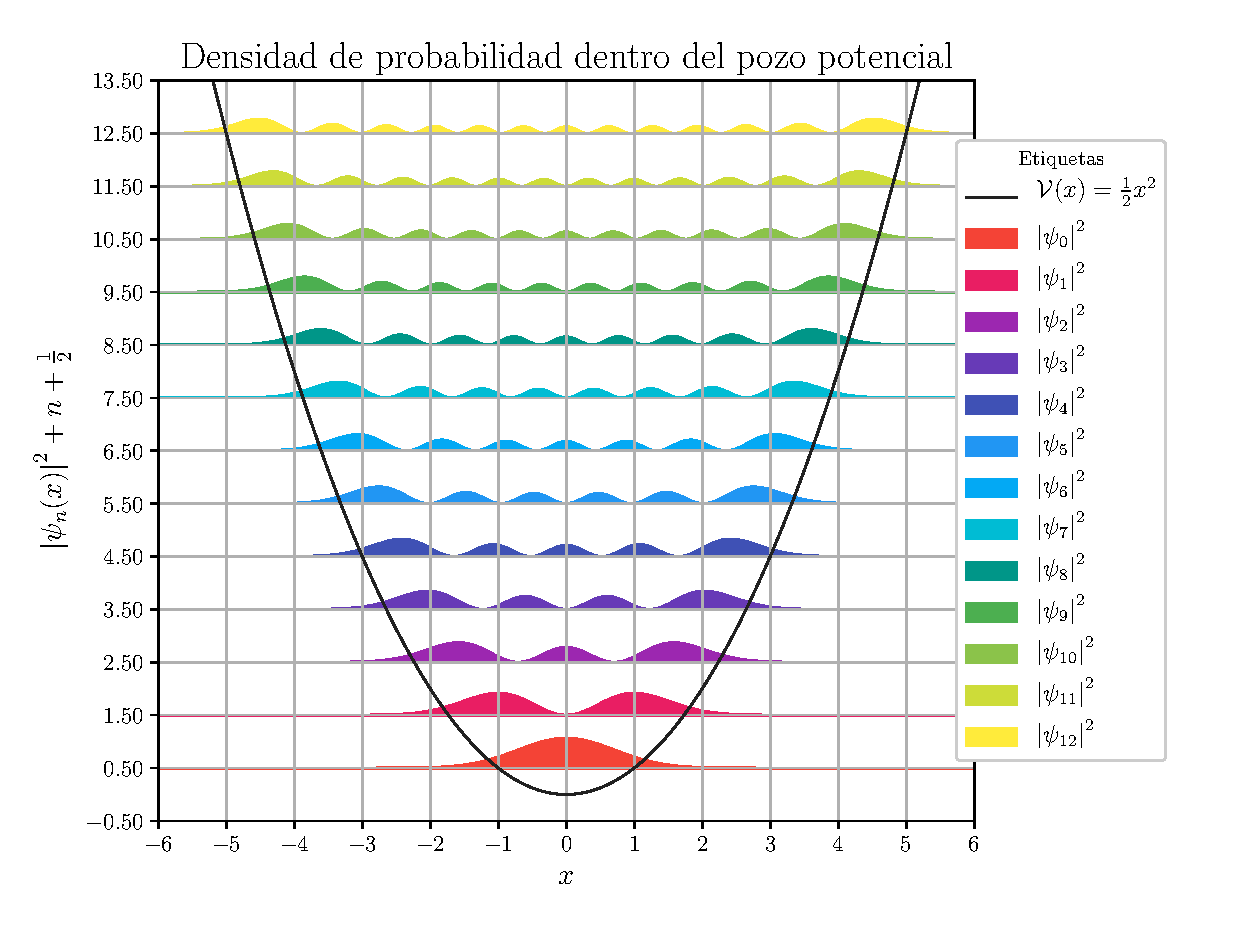
\includegraphics[scale=0.75]{Imagenes/Funciones_Normalizadas_01.eps}
\end{figure}


\end{document}